\chapter{Monsters of Athas}
\Capitalize{H}{ere} are the statistics of the monsters referenced in this book: animal companions, options for \emph{summon monster} and \emph{summon nature's ally}. For a complete description of the monsters, see \emph{Terrors of Athas}.

\section{Animal Companions}
\subsection{4th-level or higher}
\subsubsection{Baazrag}
\begin{figure}[b!]
\centering
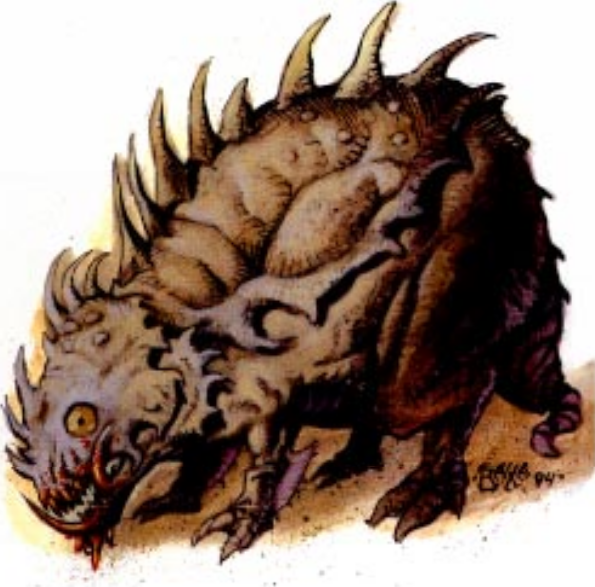
\includegraphics[width=\columnwidth]{images/boneclaw.png}
\WOTC
\end{figure}
\begin{MonsterStats}
{Small Animal}
{1d8 (4 hp)}
{+2}
{12 m (8 squares)}
{16 (+1 size, +2 Dex, +3 natural), touch 13, flat-footed 14}
{+0/+2*}
{Bite +3 melee (1d4-2 plus poison*)}
{Bite +3 melee (1d4-2 plus poison*)}
{1.5 m/1.5 m}
{Improved grab, poison}
{Low-light vision, scent}
{Fort +2, Ref +4, Will +1}
{Str 6, Dex 14, Con 10, Int 1, Wis 12, Cha 4}
{\skill{Hide} +5, \skill{Listen} +3, \skill{Spot} +6}
{\feat{Alertness}, \feat{Weapon Finesse}\textsuperscript{B}}
{Stony barrens}
{Pack (4--40)}
{\onehalf}
{None}
{Always neutral}
{2--3 HD (Small); 4--5 HD (Medium)}
{---}
\end{MonsterStats}

\textbf{Improved Grab (Ex):} If a lesser boneclaw hits with its bite it may initiate a grapple check as a free action without provoking an attack of opportunity. If it succeeds at the grapple check it may gnaw at the wound, injecting its poison. *Lesser boneclaws receive a +8 racial bonus on grapple checks.

\textbf{Poison (Ex):} Injury, Fortitude DC 10, initial damage 1d6 Con, secondary damage 1d6 Con. The save DC is Constitution-based. *Note that a lesser boneclaw can only use its poison if it successfully grapples its target.

\subsubsection{Carru}
\begin{MonsterStats}
{Large Animal}
{3d8+9 (22 hp)}
{+0}
{12 m (8 squares)}
{12 ($-1$ size, +3 natural), touch 9, flat-footed 12}
{+2/+12}
{Slam +7 melee (1d6+6)}
{Slam +7 melee (1d6+6) and gore +2 melee (1d8+3)}
{3 m/1.5 m}
{Trample 1d6+9}
{Low-light vision, scent}
{Fort +6, Ref +3, Will +2}
{Str 22, Dex 10, Con 17, Int 2, Wis 12, Cha 3}
{\skill{Spot} +4, \skill{Survival} +4}
{\feat{Alertness}, \feat{Endurance}}
{Any (Tablelands)}
{Domesticated or herd (5--50 plus 1--5 bull carrus)}
{1}
{None}
{Always neutral}
{4--5 HD (Large)}
{---}
\end{MonsterStats}

\textbf{Trample (Ex):} Reflex half DC 17. The save DC is Strength-based.
\begin{figure}[b!]
\centering
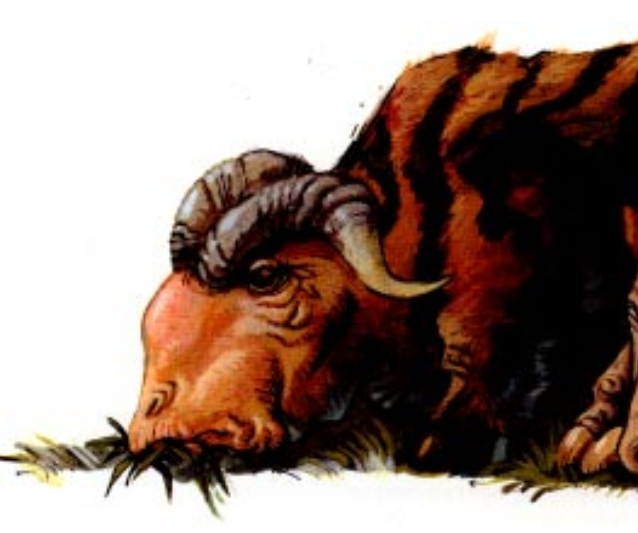
\includegraphics[width=\columnwidth]{images/carru.png}
\WOTC
\end{figure}

\vskip3cm
\subsubsection{Dire Rat}
\begin{MonsterStats}
{Small Animal}
{1d8+1 (5 hp)}
{+3}
{12 m (8 squares), climb 6 m}
{15 (+1 size, +3 Dex, +1 natural), touch 14, flat-footed 12}
{+0/$-4$}
{Bite +4 melee (1d4 plus disease)}
{Bite +4 melee (1d4 plus disease)}
{1.5 m/1.5 m}
{Disease}
{Low-light vision, scent}
{Fort +3, Ref +5, Will +3}
{Str 10, Dex 17, Con 12, Int 1, Wis 12, Cha 4}
{\skill{Climb} +11, \skill{Hide} +8, \skill{Listen} +4, \skill{Move Silently} +4, \skill{Spot} +4, \skill{Swim} +11}
{\feat{Alertness}, \feat{Weapon Finesse}\textsuperscript{B}}
{Any}
{Solitary or pack (11--20)}
{1/3}
{None}
{Always neutral}
{2--3 HD (Small); 4--6 HD (Medium)}
{---}
\end{MonsterStats}

\textbf{Disease (Ex):} Filth fever---bite, Fortitude DC 11, incubation period 1d3 days, damage 1d3 Dex and 1d3 Con. The save DC is Constitution-based.

\textbf{Skills:} Dire rats have a +8 racial bonus on \skill{Swim} checks.

Dire rats have a +8 racial bonus on \skill{Climb} checks and can always choose to take 10 on \skill{Climb} checks, even if rushed or threatened.

Dire rats use their Dexterity modifier for \skill{Climb} and \skill{Swim} checks.

\subsubsection{Eagle}
\begin{MonsterStats}
{Small Animal}
{1d8+1 (5 hp)}
{+2}
{3 m (2 squares), fly 24 m (average)}
{14 (+1 size, +2 Dex, +1 natural), touch 13, flat-footed 12}
{+0/$-4$}
{Talon +3 melee (1d4)}
{2 talons +3 melee (1d4) and bite $-2$ melee (1d4)}
{1.5 m/1.5 m}
{---}
{Low-light vision}
{Fort +3, Ref +4, Will +2}
{Str 10, Dex 15, Con 12, Int 1, Wis 14, Cha 4}
{\skill{Listen} +2, \skill{Spot} +14}
{\feat{Weapon Finesse}}
{Mountains}
{Solitary or pair}
{\onehalf}
{None}
{Always neutral}
{2--3 HD (Medium)}
{---}
\end{MonsterStats}

\textbf{Skills:} Eagles have a +8 racial bonus on \skill{Spot} checks.

\subsubsection{Erdlu}
\begin{MonsterStats}
{Medium Animal}
{2d8+2 (11 hp)}
{+2}
{12 m (8 squares)}
{13 (+2 Dex, +1 natural), touch 12, flat-footed 11}
{+1/+2}
{Claw +2 melee (1d4+1)}
{2 claws +2 melee (1d4+1) and bite $-3$ melee (1d6)}
{1.5 m/1.5 m}
{---}
{Low-light vision}
{Fort +4, Ref +5, Will +1}
{Str 12, Dex 14, Con 13, Int 2, Wis 12, Cha 3}
{\skill{Jump} +16, \skill{Listen} +5, \skill{Spot} +5}
{\feat{Alertness}}
{Any (Tablelands)}
{Solitary, pair, or flock (10-500)}
{1}
{None}
{Always neutral}
{3--4 HD (Medium); 5--6 HD (Large)}
{---}
\end{MonsterStats}

\textbf{Skills:} Erdlu receive a +10 racial bonus to all \skill{Jump} checks.

\subsubsection{Jankx}
\begin{MonsterStats}
{Tiny Animal}
{1d8+1 (5 hp)}
{+8}
{6 m (4 squares), burrow 9 m}
{16 (+2 size, +4 Dex), touch 16, flat-footed 12}
{+0/$-10$}
{Claw +6 melee (1d2$-2$ plus poison)}
{2 claws +6 melee (1d2$-2$ plus poison)}
{0.75 m/0 m}
{Poison}
{Low-light vision}
{Fort +3, Ref +6, Will +1}
{Str 6, Dex 19, Con 13, Int 1, Wis 12, Cha 4}
{\skill{Hide} +22, \skill{Listen} +8, \skill{Move Silently} +16}
{\feat{Improved Initiative}, \feat{Weapon Finesse}\textsuperscript{B}}
{Sandy wastes and stony barrens}
{Community (1-1000)}
{\onehalf}
{None}
{Always neutral}
{2 HD (Tiny); 3 HD (Small)}
{---}
\end{MonsterStats}

\textbf{Poison (Ex):} Injury, Fortitude DC 11, initial damage 1d6 Str, secondary damage 2d6 Dex. The save DC is Constitution-based.

\textbf{Skills:} Jankx receive a +10 racial bonus to \skill{Hide} and \skill{Move Silently} checks, and a +5 racial bonus to \skill{Listen} checks.

\subsubsection{Jhakar}
\begin{MonsterStats}
{Small Animal}
{2d8 (9 hp)}
{+3}
{6 m (8 squares)}
{16 (+1 size, +3 Dex, +2 natural), touch 14, flat-footed 13}
{+1/$-1$}
{Bite +5 melee (1d6$-2$)}
{Bite +5 melee (1d6$-2$)}
{1.5 m/1.5 m}
{Improved grab, pulldown}
{Low-light vision, scent}
{Fort +3, Ref +6, Will +1}
{Str 7, Dex 17, Con 11, Int 2, Wis 12, Cha 4}
{\skill{Listen} +3, \skill{Spot} +2, \skill{Survival} +3*}
{\feat{Track}, \feat{Weapon Finesse}\textsuperscript{B}}
{Any (Tablelands)}
{Solitary or pack (2--5)}
{1}
{None}
{Always neutral}
{3--4 HD (Small); 5--6 HD (Medium)}
{---}
\end{MonsterStats}

\begin{figure*}[t!]
\centering
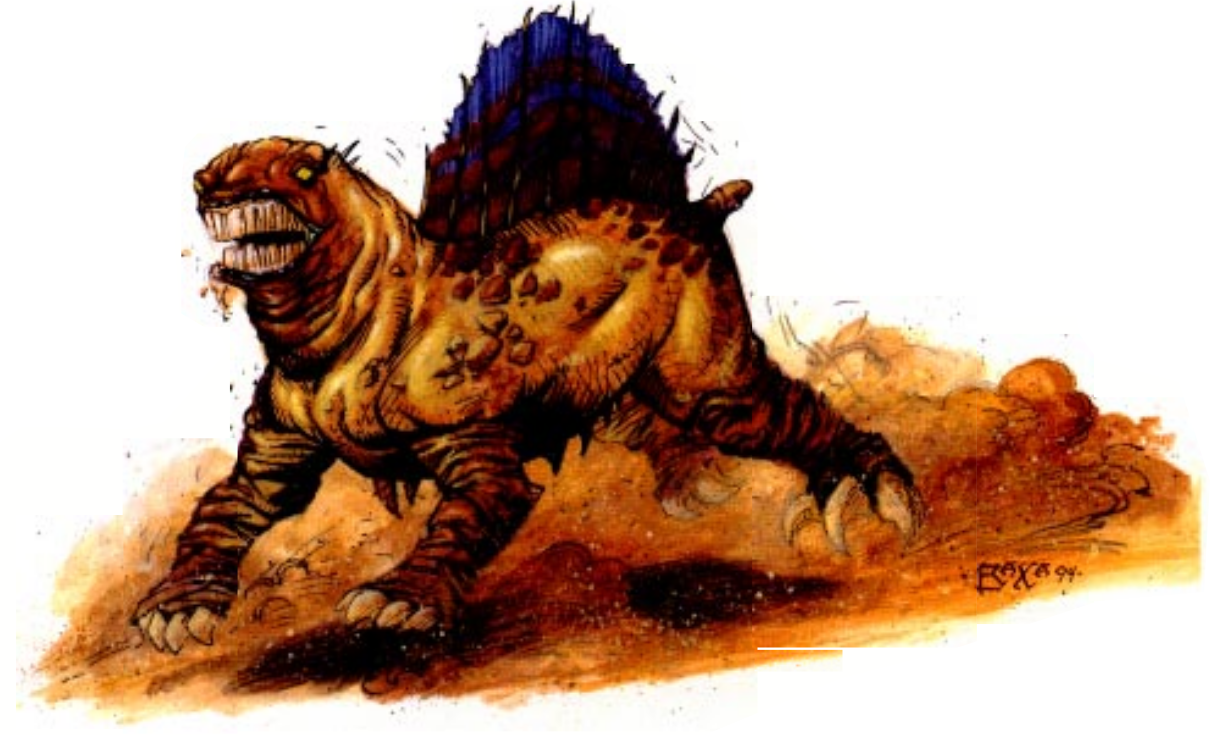
\includegraphics[width=\textwidth]{images/jhakar.png}
\WOTC
\end{figure*}

\textbf{Improved Grab (Ex):} If a jhakar hits with its bite it may initiate a grapple check as a free action without provoking an attack of opportunity. *A jhakar has a +4 racial bonus on grapple checks.

\textbf{Pulldown (Ex):} Once per round, a jhakar can either make a trip attack as a free action or aid another jhakar in a trip attack as a free action (but not both). If it wins the Strength check ($-2$ check modifier*), it may immediately make a melee attack against the tripped opponent. If the attempt fails, the opponent cannot react to trip the jhakar. *A jhakar has a +4 racial bonus on Strength checks made to trip an opponent.

\textbf{Skills:} *Jhakars receive a +4 racial bonus to Survival checks when tracking by scent.

\subsubsection{Kes'trekel}
\begin{figure}[b!]
\centering
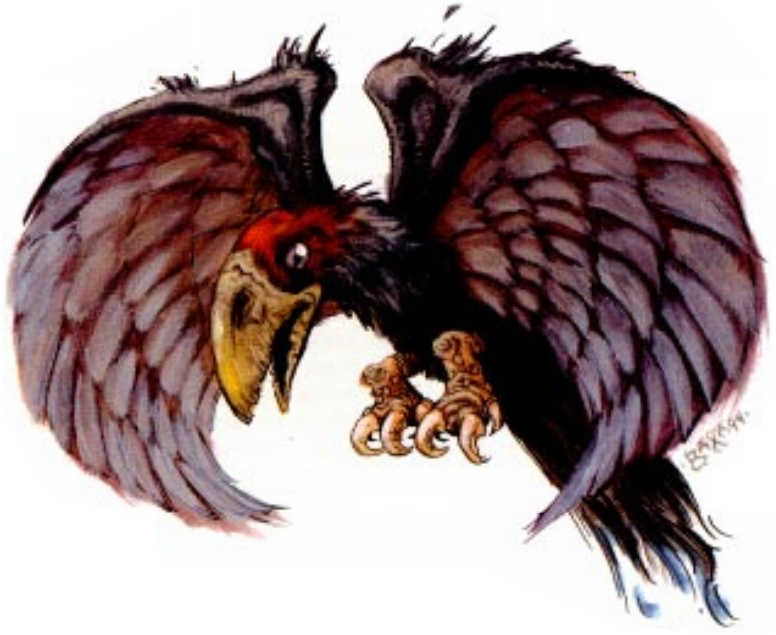
\includegraphics[width=\columnwidth]{images/kes-trekel.png}
\WOTC
\end{figure}

\begin{MonsterStats}
{Tiny Animal (Psionic)}
{1d8+1 (5 hp)}
{+1}
{3 m (2 squares), fly 18 m (average)}
{15 (+2 size, +1 Dex, +2 natural), touch 13, flat-footed 14}
{+0/$-7$}
{Bite +3 melee (1d3+1)}
{Bite +3 melee (1d3+1)}
{0.75 m/0 m}
{\emph{Aversion}}
{Low-light vision}
{Fort +3, Ref +3, Will +1}
{Str 12, Dex 12, Con 13, Int 1, Wis 12, Cha 4}
{\skill{Spot} +5}
{\feat{Flyby Attack}}
{Any}
{Flock (3--30)}
{\onehalf}
{None}
{Always neutral}
{2 HD (Small); 3--5 HD (Medium); 6--9 HD (Large)}
{---}
\end{MonsterStats}

\textit{Aversion (Ps):} A group of 20 or more kes'trekels can manifest \psionic{aversion} three times per day (Will DC 11 negates). For every 10 additional kes'trekel, increase the save DC by 1. Manifester level 3rd. The save DC is Charisma-based.

\subsubsection{Ocelot}
\begin{MonsterStats}
{Small Animal}
{1d8 (4 hp)}
{+3}
{9 m (3 squares)}
{15 (+1 size, +4 Dex), touch 15, flat-footed 11}
{+0/$-7$}
{Bite +5 melee (1d3$-2$)}
{Bite +5 melee (1d3$-2$) and 2 claws +0 melee (1d2$-2$)}
{1.5 m/1.5 m}
{Rake 1d3$-2$}
{Low-light vision, scent}
{Fort +3, Ref +3, Will +1}
{Str 7, Dex 18, Con 11, Int 2, Wis 12, Cha 4}
{\skill{Balance} +8, \skill{Climb} +4, \skill{Hide} +12*, \skill{Listen} +5, \skill{Move Silently} +8, \skill{Spot} +5}
{\feat{Alertness}, \feat{Weapon Finesse}\textsuperscript{B}}
{Scrub plains}
{Solitary, pair, or family (3--5)}
{\onehalf}
{None}
{Always neutral}
{2--3 HD (Small)}
{---}
\end{MonsterStats}

\textbf{Rake (Ex):} Attack bonus +5, damage 1d3$-2$.

\textbf{Skills:} Ocelots receive a +4 racial bonus to \skill{Balance}, \skill{Hide}, and \skill{Move Silently} checks. *In areas of tall grass or heavy undergrowth, the \skill{Hide} bonus rises to +8.

Ocelots use their Dexterity modifier for \skill{Climb} checks.

\subsubsection{Owl}
\begin{MonsterStats}
{Tiny Animal}
{1d8 (4 hp)}
{+3}
{3 m (2 squares), fly 12 m (average)}
{17 (+2 size, +3 Dex, +2 natural), touch 15, flat-footed 14}
{+0/$-11$}
{Talons +5 melee (1d4$-3$)}
{Talons +5 melee (1d4$-3$)}
{0.75 m/0 m}
{---}
{Low-light vision}
{Fort +2, Ref +5, Will +2}
{Str 4, Dex 17, Con 10, Int 2, Wis 14, Cha 4}
{\skill{Listen} +14, \skill{Move Silently} +17, \skill{Spot} +6*}
{\feat{Weapon Finesse}}
{Any (Tablelands)}
{Solitary}
{\onequarter}
{None}
{Always neutral}
{2 HD (Small)}
{---}
\end{MonsterStats}

\textbf{Skills:} Owls have a +8 racial bonus on \skill{Listen} checks and a +14 racial bonus on \skill{Move Silently} checks. *They have a +8 racial bonus on \skill{Spot} checks in areas of shadowy illumination.

\subsubsection{Snake, Small Viper}
\begin{MonsterStats}
{Small Animal}
{1d8 (4 hp)}
{+3}
{6 m (4 squares), climb 6 m, swim 6 m}
{17 (+1 size, +3 Dex, +3 natural), touch 14, flat-footed 14}
{+0/$-6$}
{Bite +4 melee (1d2$-2$ plus poison)}
{Bite +4 melee (1d2$-2$ plus poison)}
{1.5 m/1.5 m}
{Poison}
{Scent}
{Fort +2, Ref +5, Will +1}
{Str 6, Dex 17, Con 11, Int 1, Wis 12, Cha 2}
{\skill{Balance} +11, \skill{Climb} +11, \skill{Hide} +11, \skill{Listen} +7, \skill{Spot} +7, \skill{Swim} +6}
{\feat{Weapon Finesse}}
{Sandy wastes and scrub plains}
{Solitary}
{\onehalf}
{None}
{Always neutral}
{---}
{---}
\end{MonsterStats}

\textbf{Poison (Ex):} Injury, Fortitude DC 10, initial and secondary damage 1d6 Con. The save DC are Constitution-based.

\textbf{Skills:} Snakes have a +4 racial bonus on \skill{Hide}, \skill{Listen}, and \skill{Spot} checks and a +8 racial bonus on \skill{Balance} and \skill{Climb} checks.

A snake can always choose to take 10 on a \skill{Climb} check, even if rushed or threatened.

Snakes use either their Strength modifier or Dexterity modifier for \skill{Climb} checks, whichever is higher.

A snake has a +8 racial bonus on any \skill{Swim} check to perform some special action or avoid a hazard. It can always choose to take 10 on a \skill{Swim} check, even if distracted or endangered. It can use the run action while swimming, provided it swims in a straight line.

\subsubsection{Snake, Medium Viper}
\begin{MonsterStats}
{Medium Animal}
{2d8 (9 hp)}
{+3}
{6 m (4 squares), climb 6 m, swim 6 m}
{16 (+3 Dex, +3 natural), touch 14, flat-footed 14}
{+1/+0}
{Bite +4 melee (1d4$-1$ plus poison)}
{Bite +4 melee (1d4$-1$ plus poison)}
{1.5 m/1.5 m}
{Poison}
{Scent}
{Fort +3, Ref +6, Will +1}
{Str 8, Dex 17, Con 11, Int 1, Wis 12, Cha 2}
{\skill{Balance} +11, \skill{Climb} +11, \skill{Hide} +12, \skill{Listen} +5, \skill{Spot} +5, \skill{Swim} +7}
{\feat{Weapon Finesse}}
{Sandy wastes and scrub plains}
{Solitary}
{\onehalf}
{None}
{Always neutral}
{---}
{---}
\end{MonsterStats}
\textbf{Poison (Ex):} Injury, Fortitude DC 11, initial and secondary damage 1d6 Con. The save DC are Constitution-based.

\textbf{Skills:} Snakes have a +4 racial bonus on \skill{Hide}, \skill{Listen}, and \skill{Spot} checks and a +8 racial bonus on \skill{Balance} and \skill{Climb} checks.

A snake can always choose to take 10 on a \skill{Climb} check, even if rushed or threatened.

Snakes use either their Strength modifier or Dexterity modifier for \skill{Climb} checks, whichever is higher.

A snake has a +8 racial bonus on any \skill{Swim} check to perform some special action or avoid a hazard. It can always choose to take 10 on a \skill{Swim} check, even if distracted or endangered. It can use the run action while swimming, provided it swims in a straight line.

\subsection{7th-level or higher}
\subsubsection{Carru, Bull}
\begin{MonsterStats}
{Large Animal}
{6d8+24 (51 hp)}
{$-1$}
{12 m (8 squares)}
{13 ($-1$ size, $-1$ Dex, +5 natural), touch 8, flat-footed 13}
{+4/+15}
{Slam +10 melee (1d6+7)}
{Slam +10 melee (1d6+7) and gore +5 melee (1d8+3)}
{3 m/1.5 m}
{Trample 1d6+10}
{Low-light vision, scent}
{Fort +9, Ref +4, Will +1}
{Str 24, Dex 8, Con 18, Int 2, Wis 12, Cha 3}
{\skill{Listen} +3, \skill{Spot} +7, \skill{Survival} +6}
{\feat{Alertness}, \feat{Diehard}, \feat{Endurance}}
{Any (Tablelands)}
{Domesticated or herd (1--5 plus 5--50 carrus)}
{2}
{None}
{Always neutral}
{7--8 HD (Large)}
{---}
\end{MonsterStats}

\textbf{Trample (Ex):} Reflex half DC 20. The save DC is Strength-based.

\subsubsection{Cheetah}
\begin{MonsterStats}
{Medium Animal}
{3d8+6 (19 hp)}
{+5}
{15 m (10 squares)}
{15 (+4 Dex, +1 natural), touch 14, flat-footed 11}
{+2/+5}
{Bite +6 melee (1d6+3)}
{Bite +6 melee (1d6+3) and 2 claws +0 melee (1d2+1)}
{1.5 m/1.5 m}
{Trip}
{Low-light vision, scent, sprint}
{Fort +5, Ref +7, Will +2}
{Str 7, Dex 18, Con 11, Int 2, Wis 12, Cha 6}
{\skill{Hide} +6, \skill{Listen} +4, \skill{Move Silently} +6, \skill{Spot} +4}
{\feat{Alertness}, \feat{Weapon Finesse}}
{Verdant plains}
{Solitary, pair, or family (3--5)}
{2}
{None}
{Always neutral}
{4--5 HD (Medium)}
{---}
\end{MonsterStats}

\textbf{Trip (Ex):} A cheetah that hits with a claw or bite attack can attempt to trip the opponent (+3 check modifier) as a free action without making a touch attack or provoking an attack of opportunity. If the attempt fails, the opponent cannot react to trip the cheetah.

\textbf{Sprint (Ex):} Once per hour, a cheetah can move ten times its normal speed (150 meters) when it makes a charge.

\subsubsection{Crodlu}
\begin{MonsterStats}
{Large Animal}
{4d8+12 (30 hp)}
{+5}
{15 m (10 squares)}
{16 ($-1$ size, +5 Dex, +2 natural), touch 14, flat-footed 11}
{+3/+11}
{Claw +6 melee (1d6+4)}
{2 claws +6 melee (1d6+4) and bite +1 melee (1d8+2)}
{3 m/1.5 m}
{Improved grab, pounce, rake 1d6+2}
{Low-light vision}
{Fort +7, Ref +9, Will +3}
{Str 19, Dex 21, Con 17, Int 2, Wis 14, Cha 6}
{\skill{Jump} +22, \skill{Listen} +7, \skill{Move Silently} +9, \skill{Spot} +0}
{\feat{Alertness}, \feat{Endurance}, \feat{Run}\textsuperscript{B}}
{Any (Tablelands)}
{Herd (5--30)}
{3}
{None}
{Always neutral}
{5--8 HD (Large)}
{---}
\end{MonsterStats}

\textbf{Improved Grab (Ex):} To use this ability, a crodlu must hit with its bite attack. It can then attempt to start a grapple as a free action without provoking an attack of opportunity. If it wins the grapple check, it establishes a hold and can rake.

\textbf{Pounce (Ex):} If a crodlu charges, it can make a full attack, including two rake attacks.

\textbf{Rake (Ex):} Attack bonus +6 melee, damage 1d6+2.

\textbf{Skills:} Crodlu receive a +10 racial bonus on \skill{Jump} checks and a $-4$ penalty on \skill{Spot} checks.

\subsubsection{Crodlu, Heavy}
\begin{MonsterStats}
{Large Animal}
{5d8+20 (30 hp)}
{+5}
{12 m (8 squares)}
{17 ($-1$ size, +4 Dex, +4 natural), touch 13, flat-footed 13}
{+3/+13}
{Claw +8 melee (1d6+6)}
{2 claws +8 melee (1d6+6) and bite +3 melee (1d8+3)}
{3 m/1.5 m}
{Improved grab, pounce, rake 1d6+3}
{Low-light vision}
{Fort +7, Ref +9, Will +3}
{Str 22, Dex 19, Con 19, Int 2, Wis 12, Cha 7}
{\skill{Jump} +20, \skill{Listen} +7, \skill{Move Silently} +8, \skill{Spot} $-1$}
{\feat{Alertness}, \feat{Endurance}, \feat{Run}\textsuperscript{B}}
{Any (Tablelands)}
{Herd (5--30)}
{3}
{None}
{Always neutral}
{5--8 HD (Large)}
{---}
\end{MonsterStats}

\textbf{Improved Grab (Ex):} To use this ability, a heavy crodlu must hit with its bite attack. It can then attempt to start a grapple as a free action without provoking an attack of opportunity. If it wins the grapple check, it establishes a hold and can rake.

\textbf{Pounce (Ex):} If a heavy crodlu charges, it can make a full attack, including two rake attacks.

\textbf{Rake (Ex):} Attack bonus +6 melee, damage 1d6+2.

\textbf{Skills:} Heavy crodlu receive a +10 racial bonus on \skill{Jump} checks and a $-4$ penalty on \skill{Spot} checks.

\subsection{10th-level or higher}
\subsection{13th-level or higher}
\subsection{16th-level or higher}
\subsection{19th-level or higher}